\chapter[Computational Complexity]{Computational Complexity of Metropolis-Hastings Methods in High Dimensions}
\label{ch:Computational Complexity}

This chapter is devoted to the computational complexity of Metropolis-Hastings~(MH) methods applied to the target measure $ \pi^{N} $ on $ \mathbb{R}^{N} $, when $N$ is large. Informally speaking, complexity of an algorithm or a method is a measure of cost. This knowledge of computional cost of different MH~methods for certain target distribution allows to choose a suitable method for given problems. We begin by clarifying what computational complexity means to us~(Chapter~\ref{CC:Complexity}) and why there should be an optimal scaling related to complexity~(Chapter~\ref{CC:Heuristics}). To quantify optimality with respect to complexity, we introduce different criteria to measure this complexity~(Chapter~\ref{CC:Criteria}). Finally, these ideas are applied to the RWM and MALA algorithm~(Chapter~\ref{CC:Optimality and Diffusion Limits}), introduced in Chapters~\ref{MH-RWM} and~\ref{MH-MALA}, respectively and well-known results concerning simple product targets are restated. The presentation of this chapter follows the structure of~\autocite{Beskos2009, Roberts2001, Rosenthal2008}. 

\section{Complexity}
\label{CC:Complexity}

The computational complexity is an important part of the theory of the analysis of algorithms. Whereas in the first one, one tries to classify computational problems according to their inherent difficulties such that these classes are comparable to each other, the latter has the aim to determine the amount of resources (such as time and storage) necessary to execute the algorithm. Usually, the complexity or running time of an algorithm is stated as a function relating an input parameter to the number of steps (\textit{time complexity}) or storage locations (\textit{space complexity}). From a mathematical point of view, we are interested in the theoretical analysis of algorithms, i.e., we are interested in the determination of the time complexity of an algorithm in the asymptotic sense. In particular, we want to estimate the (time) complexity of the RWM and MALA algorithm applied to the target measure $ \pi^{N} $, when the dimension $N$ tends to infinity. Considering the two Algorithms~\ref{Algo-RWM} and~\ref{Algo-MALA} with their respective proposal and acceptance-rejection step, the cost of each iteration can usually be computed as a function of dimension by simple means. Thus, the question of computational complexity boils down to understanding the number of steps required to explore the target $ \pi^{N} $.


This exploring of the target distribution is usually divided into two phases: the \textit{transient} and the \textit{stationary} phase. Specifically, transient phase means that we do not assume the initial value is distributed according to the target distribution. In particular, we consider Metropolis-Hastings algorithms, which start out far in the ``tails'' of $ \pi^{N} $, such that the generated Markov chains have to approach the ``center'' of $ \pi^{N} $. Conversely, the stationary phase is characterized by the fact that the initial value of the chain or algorithm is distributed according to the target distribution $ \pi^{N} $. Following the approach of Roberts and coworkers initialized by the pair of papers~\autocite{Roberts1997, Roberts2001}, we focus on the analysis of the stationary phase in the sequel. Nevertheless, an analysis of the transient phase of different Metropolis-Hastings methods can be found in~\autocite{Christensen2003, Jourdain2013}.




\begin{figure}%[htb]
 \begin{center} 
 
  \begin{subfigure}{.5\textwidth}
    \centering
    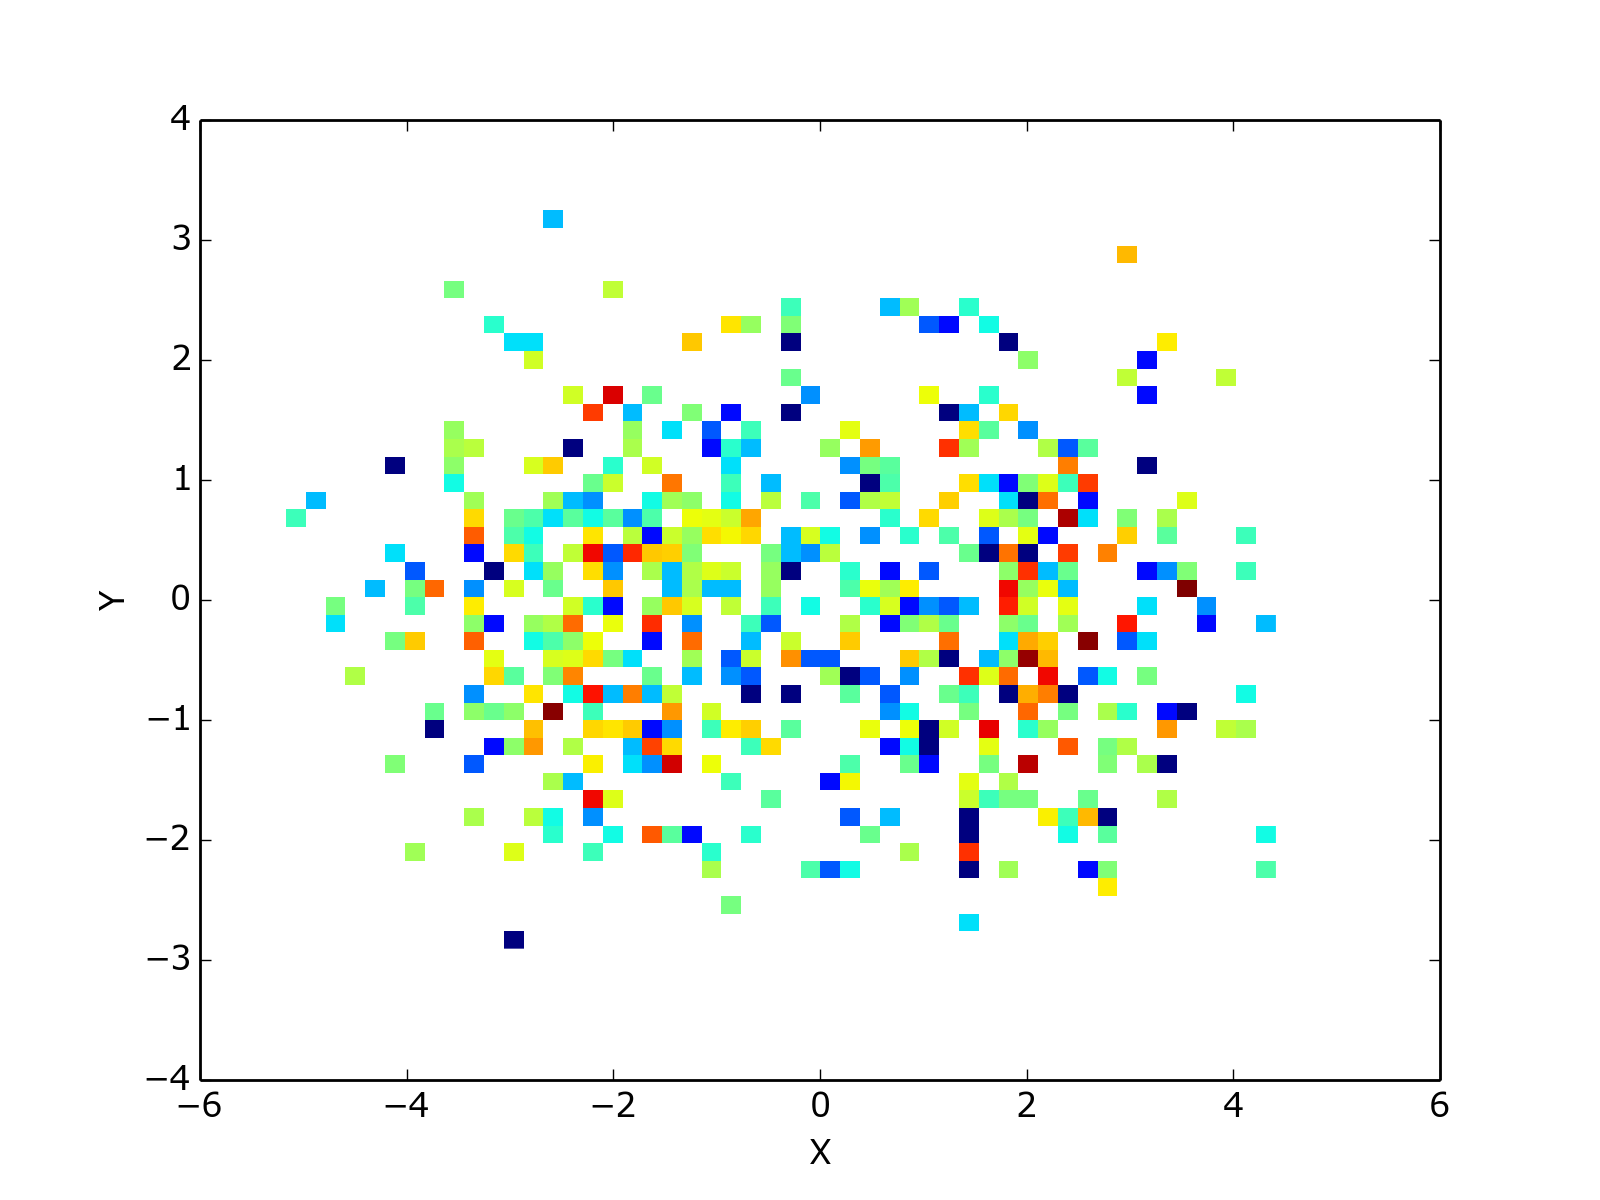
\includegraphics[width=\textwidth]{figure_CC_RWM_large_Histo}
  \end{subfigure}%
  \begin{subfigure}{.5\textwidth}
    \centering
    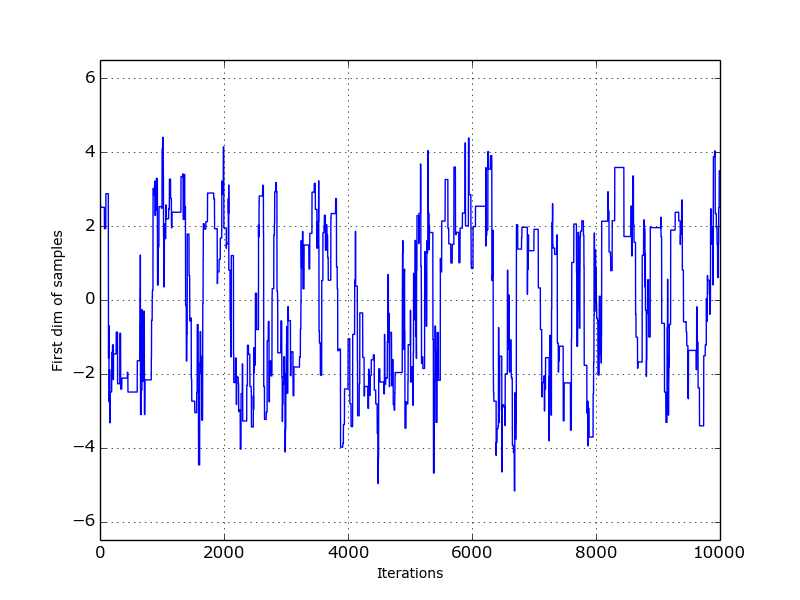
\includegraphics[width=\textwidth]{figure_CC_RWM_large_2}
  \end{subfigure}
  \vspace*{1mm}
  \subcaption{A simulation with a very large proposal variance $ \sigma^2 $.}
  \label{fig:HeuristicHistoPlotRWM-large}
  \vspace*{3mm}
  
  
  \begin{subfigure}{.5\textwidth}
    \centering
    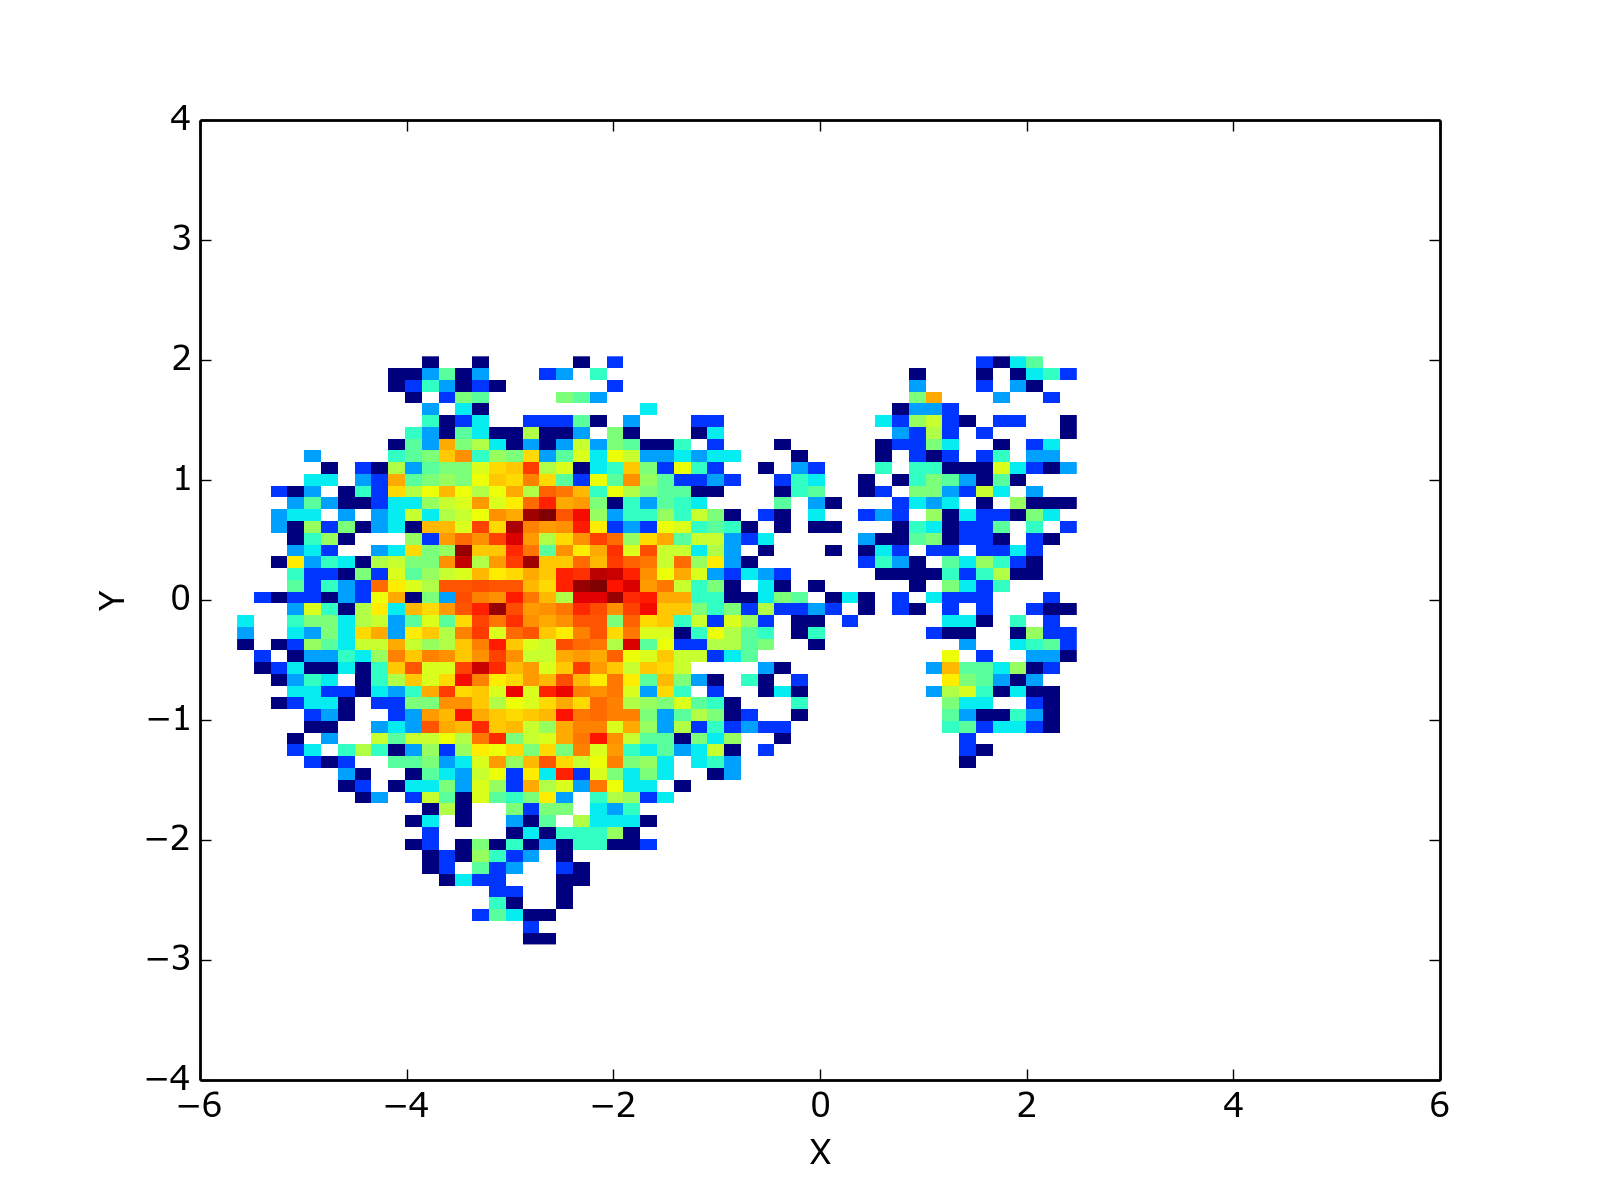
\includegraphics[width=\textwidth]{figure_CC_RWM_small_Histo}
  \end{subfigure}%
  \begin{subfigure}{.5\textwidth}
    \centering
    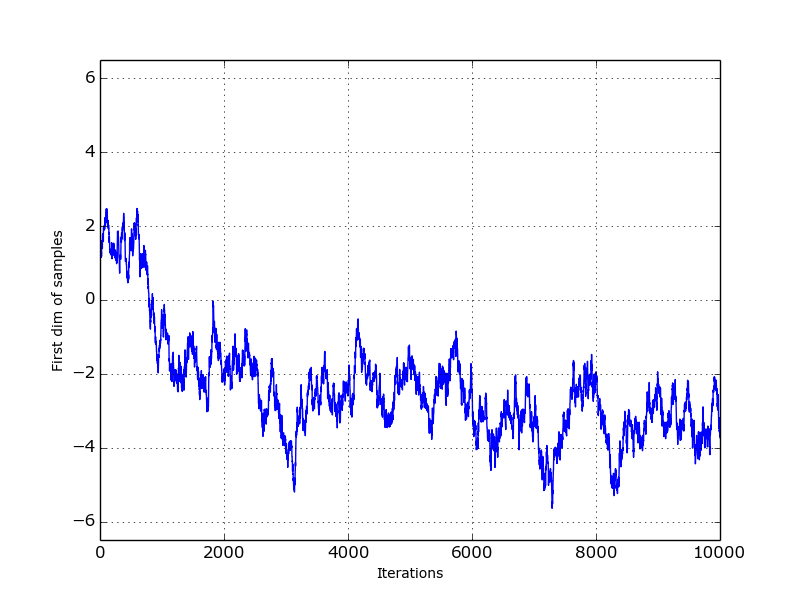
\includegraphics[width=\textwidth]{figure_CC_RWM_small_2}
  \end{subfigure}
  \vspace*{1mm}
  \subcaption{A simulation with a very small proposal variance $ \sigma^2 $.}
  \label{fig:HeuristicHistoPlotRWM-small}
  \vspace*{3mm}
  
  \begin{subfigure}{.5\textwidth}
    \centering
    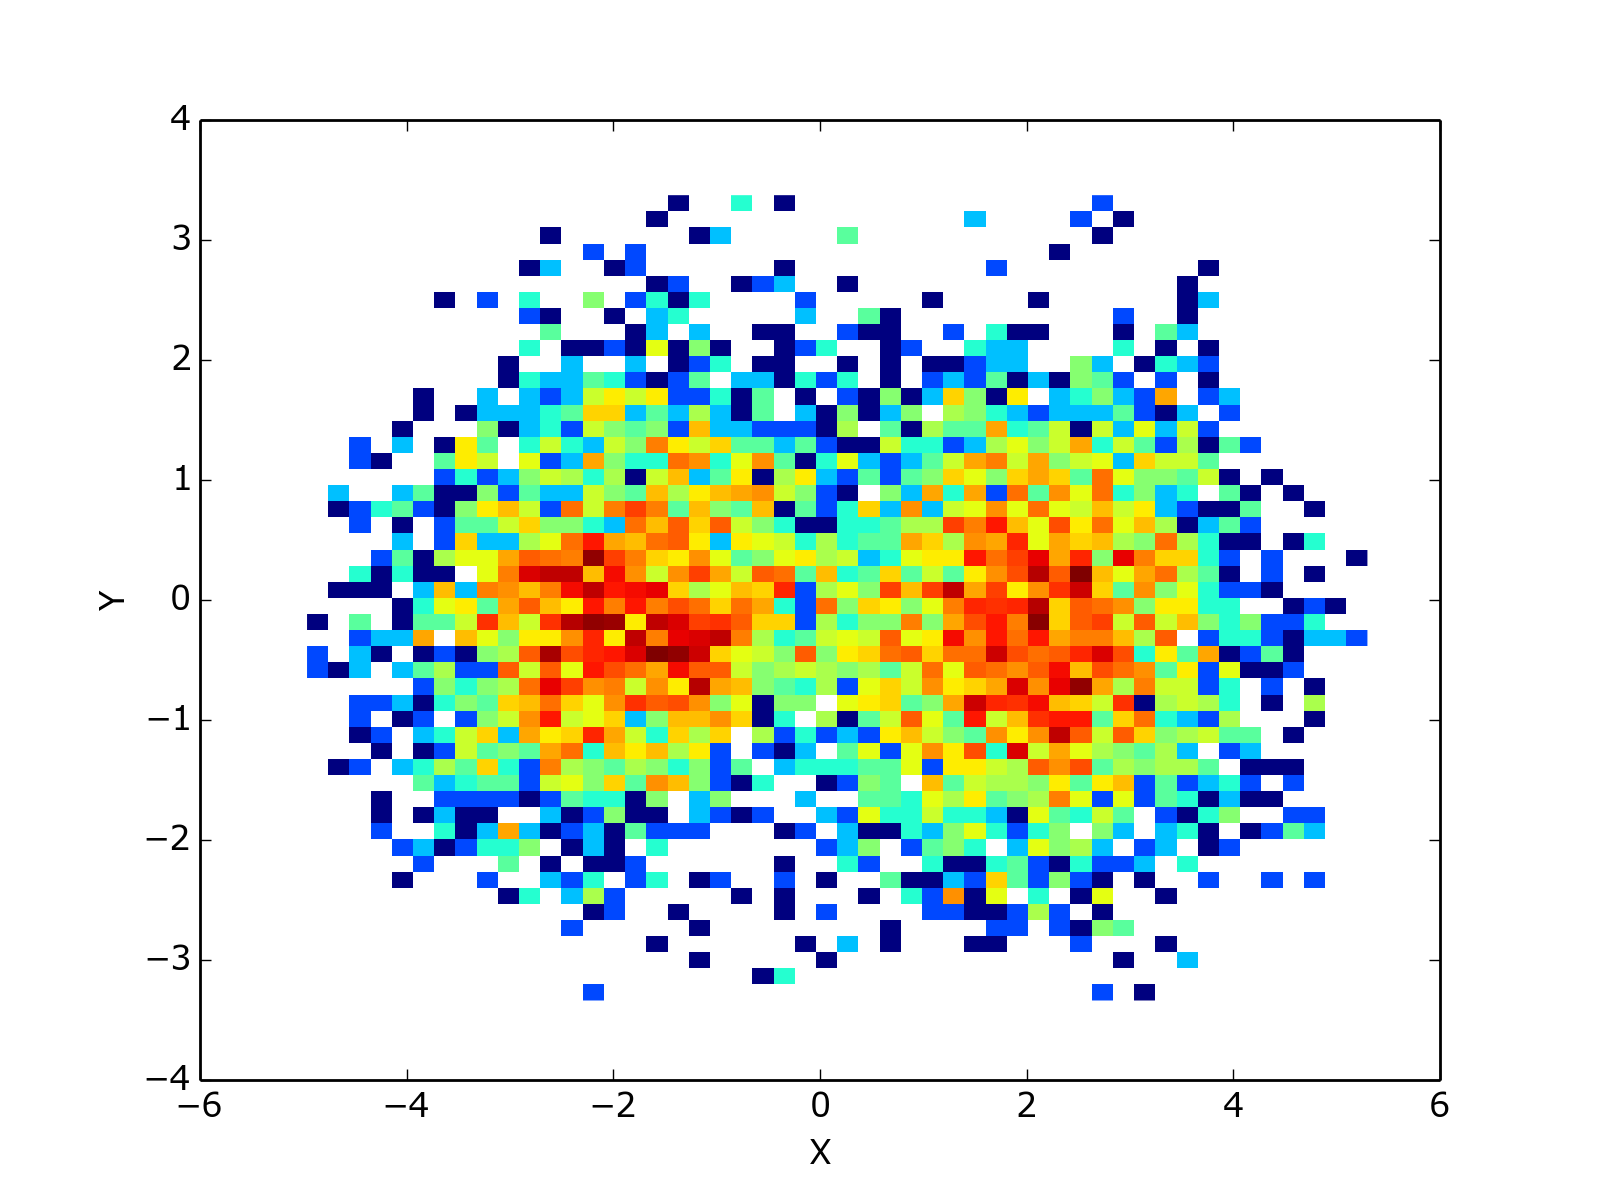
\includegraphics[width=\textwidth]{figure_CC_RWM_inter_Histo}
  \end{subfigure}%
  \begin{subfigure}{.5\textwidth}
    \centering
    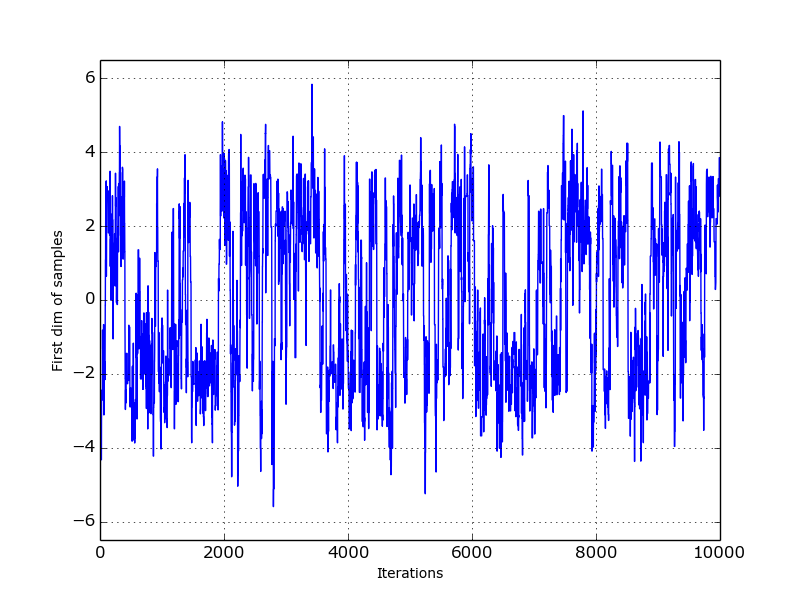
\includegraphics[width=\textwidth]{figure_CC_RWM_inter_2}
  \end{subfigure}  
  \vspace*{1mm}
  \subcaption{A simulation with an intermediate proposal variance $ \sigma^2 $.}
  \label{fig:HeuristicHistoPlotRWM-medium}
  
 \end{center}
 
  \caption{Histograms and trace-plots of three different simulations of RWM in dimension $N=5$ for for a two modal Gaussian standard distribution with 10,000 iterations.}
  \label{fig:HeuristicHistoPlotRWM}
\end{figure}


\section{Heuristic Argument for an Optimal Scaling}
\label{CC:Heuristics}

In this section, we briefly want to give an heuristic argument for the existence of an optimal scaling of the proposal variance $ \sigma^2 (N) $ of Metropolis-Hastings algorithms.
We consider a simple example to illustrate the issues of choosing an appropriate proposal variance. Suppose that the target distribution $ \pi^{N} $ is a two modal Gaussian in dimension $N=5$, i.e., the sum of two standard Gaussian distributions with half its mass at $ m^+ = (2,0,0,0,0)^T $ and  $ m^- = (-2,0,0,0,0)^T $. Moreover, we use the RWM Algorithm~\ref{Algo-RWM} with Gaussian proposals to sample from $ \pi^{N} $, where $ \sigma^2 $ denotes the proposal variance. This target measure~$\pi^N$ is a simple but non-trivial example of a multidimensional probability distribution as the first component is not a scaled version of the other components. These two peaks in the first dimension cause a challenge for the algorithm since it has to pass through the tunnel near zero to reach the other peak. Therefore, it is a good example to examine the performance of the MCMC methods as simple trace-plots and 2D-histograms give a comprehensible insight wether the algorithms are well performing or not.

In Figure~\ref{fig:HeuristicHistoPlotRWM}, the results of three different simulations with 10,000 iterations each are shown. On the left hand side of each of the histograms of the simulation the color red represents a high number of samples, whereas the color blue indicates that few samples are being detected in that area.  A good histogram of the considered two-modal Gaussian should look like Figure~\ref{fig:HeuristicHistoPlotRWM-medium}. On the histograms' right hand sides, the traceplot of the first coordinate of each iteration is given. A simulation which explores the first dimension of the two-modal Gaussian target effectively, should oscillate frequently between the two modes minus four and plus four. It is intuitively clear that we can make the performance of the algorithm arbitrarily poor by choosing $ \sigma^2 $ either very small or very large. For extremely large values of $ \sigma^2 $ the algorithm will very often propose large jumps to regions where the target distribution $ \pi^{N} $ is extremely small. Therefore, most of these proposals will be rejected and the algorithm stays fixed for large numbers of iterations. On the other hand, if $\sigma^2$ is taken to be very small, the algorithm will propose small jumps. Almost everyone of these jumps will be accepted as the acceptance probability $ \alpha^{N} $ is near to one. Nevertheless the size of the jumps is too small for the generated Markov chain to explore the space of the target distribution rapidly. Hence the algorithm will take a long time to converge to stationarity. Conversely, for intermediate values of the proposal variance $\sigma^2$, the algorithm performs quite effectively. Thus the computional complexity for this simulation should be smaller. This is illustrated in Figure~\ref{fig:HeuristicHistoPlotRWM-medium}.

Both extremes are avoided rather effectively by  monitoring the \textit{acceptance rate} of the algorithm, i.e., the fraction of proposed moves which are accepted. If this fraction is very close to zero, this suggests that the $ \sigma^2 $ is too large (as in Figure~\ref{fig:HeuristicHistoPlotRWM-large}). If this fraction is very close to one, this suggests that $ \sigma^2 $ is too small (as in Figure~\ref{fig:HeuristicHistoPlotRWM-small}). Having an acceptance rate far from both, zero and one, we avoid both extremes (as in Figure~\ref{fig:HeuristicHistoPlotRWM-medium}), which leads to a better performance of the algorithm. This principle of choosing an appropriate proposal variance applies for all dimensions $N$ and for the MALA algorithm, too. However, such an effective intermediate value for $\sigma^2$ decreases when the dimension increases, see e.g., Figure~\ref{fig:proposalVarianceForDimensions} in Chapter~\ref{sec:introduction}. 


Since we want to analyze the behavior or scale of such an appropriate proposal variance~$\delta(N)$ for Metropolis-Hastings methods depending on the dimension~$N$, we call such a choice of optimal~$\delta(N)$ an \textit{optimal scaling} of the MCMC algorithm. Therefore, we have to rate the performance of MCMC algorithms. In the following sections, we want to give a more formal understanding of when a Markov chain explores the target distribution effectively.





\section{Criteria for Optimal Scaling}
\label{CC:Criteria}

We emphasize that our aim is to estimate the computational complexity of Metropolis-Hastings algorithms exploring a target distribution when started in stationarity. The arising question is how to measure the quality of exploring a distribution. We will present four criteria, any of which has the capacity to measure whether a Markov chain explores the target distribution or not. 

Assume that $ x^{0,N}  \thicksim \pi^{N} $ and that the $\pi^{N}$-invariant Markov chain $ x^{N} := \left\{ x^{k,N}\right\}_k $ is generated according to the RWM or MALA algorithm. Recall that $ y^{k,N} $ denotes the possible next candidate in the $k$-th step for the respective proposal transition density $ q(x,y) $ and that the Metropolis-Hastings acceptance probability, as defined in Equation~(\ref{MH-Acceptance probability definition}), is given by $ \alpha^{N}\left(x^{k,N},y^{k,N}\right) $. Moreover, we want to recall that the RWM as well as the MALA algorithm depend on the parameter $ \sigma^2 > 0 $, which is called the proposal variance or discret time increment and it depends on the dimension $N$. Then the four criteria are:

\begin{enumerate}
 \item choose the proposal variance $ \sigma^2 $ to maximize the \textit{expected mean square jump distance}
 \begin{equation}
  \label{CC:Mean Square jump distance}
  \mathbb{E}\left[ \left\| x^{k+1,N} - x^{k,N}  \right\|^2 \right];
 \end{equation}
 
 \item choose the proposal variance $ \sigma^2 $ to maximize the \textit{mean time-step}
 \begin{equation}
  \label{CC:mean time-step}
  \sigma^2 \times \mathbb{E}\left[ \alpha^{N}\left(x^{k,N},y^{k,N}\right) \right];
 \end{equation}
 
 \item choose the proposal variance $ \sigma^2 $ maximal subject to the constraint that the \textit{average acceptance probability} is bounded away from zero, uniformly in dimension $N$
 \begin{equation}
  \label{CC:average acceptance probability}
  \liminf_{N \to \infty} \mathbb{E} \left[  \alpha^{N}\left(x^{k,N},y^{k,N}\right) \right] > 0;
 \end{equation}
 
 \item choose the proposal variance $ \sigma^2 $ maximal for which there exists a $ \pi^{N} $-invariant \textit{diffusion limit} of the continuous interpolation
 \begin{equation}
  \label{CC:Continuous interpolation}
  z^{N}(t) := \left( \frac{t}{\Delta t} -k \right) x^{k+1,N} + \left( k+1 - \frac{t}{\Delta t} \right) x^{k,N} \qquad \text{ for } k \Delta t \leq t < (k+1)\Delta t 
  \end{equation}
  as $N$ tends to infinity, where we chose the scale of the interpolation to satisfy $ \Delta t := l^{-1} \sigma^2  $, with the parameter $l$ a \textit{tuning} parameter which is independent of the dimension $N$.
 
\end{enumerate}

In all four cases it is natural to deduce that the number of Markov chain steps
required in stationarity is inversely proportional to the proposal variance $ \sigma^2 $ which in turn depends on the dimension $N$. This will be the concept to determine an optimal scaling of a Metropolis-Hastings method depending on the dimension $N$. More precisely, we are seeking for every~$N$, a \textit{scaling} in terms of the proposal variance~$ \sigma^2 = \sigma^2 (N) $ which is optimal according to at least one of these \textit{mixing} criteria.

\begin{rem}\label{rem:other criteria}
Nevertheless, further criteria to find \textit{better} or \textit{best} MCMC methods that focus on other aspects than \textit{exploring the space}. Possible choices include the convergence rates of the transition kernels of the generated Markov chains and the variance and integrated autocorrelation time of the chains, which depend strongly on the target distribution $ \pi^{N} $. See~\autocite{Rosenthal2008} for further reference. Note that the choice of an appropriate criterion depends on the specific question being asked. 
\end{rem}

In the following section, we will discuss the relations among these four \textit{mixing} criteria. We will see that in some circumstances, these different definitions are all equivalent (including further criteria as mentioned in Remark~\ref{rem:other criteria}), leading to uniformly optimal choices of the algorithm parameter $\sigma^2$.


\section{Optimality and Diffusion Limits}
\label{CC:Optimality and Diffusion Limits}

In this section, we now turn to the subject of diffusion limits. More precisely, we will link all four presented \textit{mixing} criteria, if a diffusion limit exists for the continuous interpolant of the Markov chain given in Equation~(\ref{CC:Continuous interpolation}). In this case, all optimality criteria will be asymptotically equivalent for the dimension $N$ tending to infinity and the main issue will be to identify the circumstances under which such a diffusion limit exists.

The general idea is as follows. First of all, we set the scaling of the interpolation (Equation~(\ref{CC:Continuous interpolation})) and the proposal variance. Considering 
\begin{equation}
\label{CC:Choice of scaling gamma}
  \Delta t = N^{-\gamma} \text{ for } \gamma > 0,                                                                                                                                                                                                                                                                                                                       \end{equation}
we obtain for the proposal variance $ \sigma^2 (N) = l\;N^{-\gamma} $, with $l$ a \textit{tuning} parameter and $ \gamma $ the \textit{scaling} parameter both independent of the dimension $N$. The main issue is now to choose $l$ and $\gamma$. We choose the scaling parameter $\gamma$ such that the interpolant $ z^{N} $ converges weakly to a suitable stationary diffusion process denoted by $z$ for a specific scaling parameter $\gamma$. Then it is natural to deduce that the number of Markov chain steps required in stationarity is inversely proportional to $ \Delta t $ and so grows like $ N^{\gamma} $. In other words, smaller values for $\gamma$ result in better asymptotic complexity. Additionally, we choose the tuning parameter $l$ in the following way. The theory of diffusions allows us to set a time-scale for the limit diffusion $z$, which is often called the \textit{speed measure}. This speed measure has a parametric dependence on the tuning parameter $l$ and it can be choosen maximal depending on $l$. The concrete choice of the parameter~$l$ will be done in the end after deriving the diffusion limit.

Furthermore, the existence of a diffusion limit for an appropriate $ \gamma > 0 $ shows that all optimality criteria coincide. For a more detailed overview see \autocite{Beskos2009}. For practical relevance, we derive an universal [independent of the target distribution] asymptotically optimal acceptance probability from the choice of the tuning parameter $l$ and the corresponding speed measure.

\begin{rem}
\label{rem:finite dimension}
 This approach leads to an asymptotic assertion for the optimal scaling of RWM and MALA algorithms as dimension $N$ tends to infinity. Nevertheless, numerical studies (e.g., \autocite{Gelman1996, Roberts2001} and Chapter~\ref{Numerical Results}) indicate that this asymptotic behavior does seem to fit finite-dimensional situations for $N$ bigger than five well.
\end{rem}

In the end, the crucial point is to identify such limit diffusion processes and the two tuning and scaling parameters $l$ and $\gamma$. This is exactly the ansatz of the research programm initiated by Roberts and coworkers in the pair of papers~\autocite{Roberts1997, Roberts2001}. Thus, we want to  briefly present the results for some simple target distributions $ \pi^{N} $.


\subsection{Existing Diffusion Limit Results}
\label{CC:Existing results}

The aim of this section is to review some previous results and to give an overview for which classes of target distributions $\pi^{N}$ optimal scaling results due to diffusion limits have been achieved. We focus mainly on the work of  Gelman, Gilks, Roberts and Rosenthal and B\'{e}dard \autocite{Bedard2007, Roberts1997, Roberts2001, Roberts1998}. Further work includes optimal scaling for the MALA algorithm for nonproduct targets in the context of nonlinear regression \autocite{breyer2004} and optimal scaling tor the transient phase of the RWM and MALA algorithm \autocite{Christensen2003, Jourdain2013}.

\subsubsection{I.i.d.\,Product Targets} 

The simplest class of target measures for which the analysis can be carried out are target distributions $ \pi^{N} $ of the form

\begin{equation}
 \label{CC:iid product targets}
 \frac{d \pi^{N}}{d \lambda^{N}}(x) = \prod_{i=1}^{N} f(x_i).
\end{equation}
Here $ \lambda^{N} $ denotes the $N$-dimensional Lebesgue measure, and $f(x)$ is a one-dimensional probability density function. Hence $\pi^{N}$ has the form of an independent and identically distributed~(i.i.d.) product. This class of target distributions was first analyzed in \autocite{Roberts1997} for the RWM and in \autocite{Roberts1998} for MALA. They used Gaussian jump proposals for the Random Walk proposals (obtained from the discrete approximation of Brownian motion as described in Chapter~\ref{MH-RWM})
\begin{equation}
 \label{CC:RWMPoposals}
 y = x + \sqrt{\sigma^2}\,Z^{N}, \qquad Z^{N} \thicksim \mathcal{N}\left( 0,I_N \right),
\end{equation}
and the Langevin proposal (obtained from the time discretization of the Langevin diffusion as described in Chapter~\ref{MH-MALA})
\begin{equation}
 \label{CC:MALAProposals}
 y = x + \frac{1}{2} \sigma^2 \nabla \log \pi^{N} (x) + \sqrt{\sigma^2} Z^N, \qquad Z^{N} \thicksim \mathcal{N}\left( 0,I_N \right).
\end{equation}
Here $\sigma^2 $ denotes the proposal variance as before.  For the $N$-dimensional target $\pi^{N}$ defined in Equation~(\ref{CC:iid product targets}), they defined a speeded up continuous interpolant for the generated Metropolis-Hastings Markov chains $ x^{N} = \left\{ x^{k,N}\right\}_{k \geq 0} $ as follows
\begin{equation}
\label{CC:Continuous interpolant 2}
 z^{N}(t) := \left( \frac{t}{\Delta t} -k \right) x^{k+1,N} + \left( k+1 - \frac{t}{\Delta t} \right) x^{k,N} \qquad \text{ for } k \Delta t \leq t < (k+1)\Delta t.
\end{equation}
They chose the proposal variance to satisfy $ \sigma^2 = l \Delta t $, with $ \Delta t = N^{-\gamma} $ as described in Section~\ref{CC:Criteria}, where the scaling parameter $\gamma$ depends on the choosen algorithm. To avoid repetition when stating results for RWM and MALA we define the following values for the scaling parameter:
\begin{align}
 \text{RWM: } & \; \gamma = \gamma^{RWM} = 1, \\
 \text{MALA: } & \; \gamma = \gamma^{MALA} = \frac{1}{3}.
\end{align}
As usual in mathematics, there is a different order to proving something and writing it down. Obviously, these values for~$\gamma$ represent the desired scaling parameters one wishes to obtain for the RWM and MALA algorithm but to state the results, one needs them in the beginning.

It was shown for the RWM and MALA algorithms that the projection of $z^{N}$ onto any single fixed coordinate direction $x_i$ converges weakly in $ C \left( [0,T];\mathbb{R} \right) $ to $z$, the scalar limit diffusion process
\begin{equation}
 \label{CC:Scalar Limit Diffusion}
 \frac{dz}{dt} = \frac{1}{2} h(l) \left( \log f(z) \right)' + \sqrt{h(l)}\frac{d\mathcal{W}}{dt}
\end{equation}
for $ h(l) > 0 $, a constant determined by the tuning parameter $l$, and $ \mathcal{W} $ a standard Brownian motion in $ \mathbb{R}^{N} $.
More precisely, under a number of smoothness conditions on the density $f$ in (\ref{CC:iid product targets}), the following (composed) result holds as stated in~\autocite{Roberts1997} for RWM and in~\autocite{Roberts1998} for MALA.

\begin{thm}
 \label{CC: Product Diffusion Limit Result}
 
 Consider a Metropolis-Hastings chain $ x^{N} = \left\{  x^{k,N} \right\}_{k} $ for a target distribution having the density $ \pi^{N} $ of the form (\ref{CC:iid product targets}) and with either RWM proposals as in (\ref{CC:RWMPoposals}) or MALA proposals as in (\ref{CC:MALAProposals}) for dimension $N$.
 
 Let $ \sigma^2 (N) = l\,N^{-\gamma}$ and define the piecewise linear continuous interpolant $z^{N}$  as in (\ref{CC:Continuous interpolant 2}) according to the different scaling of $\gamma$. Consider the projection of $z^{N}$ onto any single fixed coordinate direction $x_i$. Then $z^{N}(t)$ converges weakly in $ C \left( [0,T]; \mathbb{R}^{N}\right) $ to the scalar diffusion process $z(t)$ given by (\ref{CC:Scalar Limit Diffusion}), where the 'speed function' $h(l)$ is given by
 \begin{align}
  h^{RWM}(l) = & \; l \cdot 2 \Phi \left( - \frac{1}{2} I l^{1/2} \right), \\
  h^{MALA}(l) = & \; l \cdot 2 \Phi \left( - J l^{3/2} \right),
 \end{align}
 with $\Phi$ being the standard normal cumulative density function and
 \begin{align}
  I := & \; \mathbb{E} \left[ \left( \left( \log f \right)' \right)^2  \right]^{1/2}, \\
  J := & \; \mathbb{E} \left[ \frac{1}{48} \left( 5 \left( \left( \log f \right)''' \right)^2 - 3 \left( \left( \log f \right)'' \right)^3 \right) \right]^{1/2},
 \end{align}
 where the expectations are taken with respect to $f$.
 
\end{thm}

The quantities $I$ and $J$ can be interpreted as measures of the roughness of the target and therefore depend strongly on $f$. The quantities 
\begin{equation}
 2 \Phi \left( - \frac{1}{2} I l^{1/2} \right) \quad \text{ and } \quad 2 \Phi \left( - J l^{3/2} \right)
\end{equation}
correspond to the asymptotic average acceptance probability as shown in \autocite{Roberts1997} and \autocite{Roberts1998}, respectively.
We now explain the following two important implications of this result:

\begin{enumerate}
 \item Since time has to be accelerated in the interpolant by a factor $ \left( \Delta t \right)^{-1} = N^{\gamma}$ in order to observe a convergence to a diffusion limit, we can conclude that in stationarity the exploration of the invariant measure scales as $ \mathcal{O}(N^{\gamma}) $. Particularly, the RWM algorithm scales as $ \mathcal{O}(N) $ and the MALA algorithm scales as $ \mathcal{O}(N^{1/3}) $.
 \item The speed at which the invariant measure is explored, when started in stationarity, is maximized by choosing $l$ in such a way that  $h(l)$ is maximized. This optimal choice of~$l$ depends on $I$ and $J$, respectively, and leads to an optimal value for the asymptotic average acceptance probability~$\alpha(l)$. Writing the speed measure~$h(l)$ as a function depending on~$\alpha(l)$, the dependence on $I$ and $J$ cancels out and both optimal values for~$h(l)$ and~$\alpha(l)$ are therefore independent of $f$, see \autocite{Roberts1997} and \autocite{Roberts1998}. This optimal diffusion speed~$h(l)$ is achieved at an asymptotic average acceptance probability of 0.234 for  RWM and 0.574 for MALA (rounded to three decimals).
\end{enumerate}

We note that the MALA algorithm has a better computional complexity ($ \mathcal{O}(N^{1/3}) $ instead of $ \mathcal{O}(N) $) and a larger asymptotic average acceptance probability (0.574 instead of 0.238), as compared to RWM algorithms. This result is not surprising as the MALA algorithm incorporates more information on the target distribution in the form of $ \nabla \log \pi^{N}(x) $ which on the other hand has to be calculated in each step of the algorithm. In other words, the MALA provides more sophisticated proposals that lead to better an exploration of the target distribution and less rejections. We recall again that although these results are asymptotically, numerical studies indicate that these optimality conditions hold also for finite dimensions, see Remark~\ref{rem:finite dimension}.

\begin{rem}
\label{rem:Conditions on f}
 The (sufficient) regularity conditions needed for this result rely on smoothness conditions on the function $\log f$. Essentially, for the RWM algorithm $\log f$ is assumed to be twice continuously differentiable whereas for the MALA algorithm the existence of eight continuous derivatives of $\log f$ is assumed. The details of sufficient conditions can be found in~\autocite{Roberts1997} for RWM and in~\autocite{Roberts1998} for MALA.
\end{rem}





\subsubsection{Hierachical and Scaled Product Targets} 

These first results for RWM and MALA algorithms for i.i.d.\,product targets have been extended to a (slightly) larger class of target measures. Consider the  \textit{scaled product targets} of the form

\begin{equation}
 \label{CC:Scaled product targets}
 \frac{d \pi^{N}}{d \lambda^{N}}(x) = \prod_{i=1}^{N} C_i f(C_i x_i),
\end{equation}
where $f$ is again a fixed one-dimensional density (satisfying the same assumptions as before, see Remark~\ref{rem:Conditions on f}), but where now there is a scaling factor $C_i > 0$ in each component.

Roberts and Rosenthal~\autocite{Roberts2001} and B\'{e}dard~\autocite{Bedard2007} considered different assumptions on the scaling factors $ C_i $'s, but all proved that the results concerning the optimal scaling and tuning of the asymptotic average acceptance probability of the i.i.d. product targets extend to this class of scaled and hierachical non-i.i.d. products. We have to note that B\'{e}dard~\autocite{Bedard2007} only considered the RWM algorithm for the hierachical targets whereas Roberts and Rosenthal~\autocite{Roberts2001} proved their results for both RWM and MALA algorithm for the scaled inhomogeneous targets.
The main idea of scaling the interpolant of the generated Metropolis-Hastings Markov chain by $\gamma$ such that it converges to a diffusion process and tuning the speed measure of this limit diffusion by $l$ is similar as in the case of i.i.d. product targets. Therefore, we only want to emphasize the different assumptions on the scaling factors $C_i$ and refer for further details to~\autocite{Bedard2007, Roberts2001}.


Roberts and Rosenthal~\autocite{Roberts2001} consider independent and identically distributed scaling factors $C_i$ with a normalized mean $\mathbb{E}[C_1] = 1$ and a finite variance $ \mathbb{E}[C_1^2] = b < \infty $. Although the MCMC algorithms will be slowed down in comparison to the homogeneous targets as in Equation~(\ref{CC:iid product targets}), the optimal scale of $\mathcal{O}(N)$ for RWM and $ \mathcal{O}(N^{1/3}) $ for MALA holds. In particular, the optimal average acceptance probabilities are still equal to 0.234 for RWM and 0.574 for MALA, respectively.


A more complex setup is the following taken from~\autocite{Bedard2007}. Consider targets of the form given in Equation~(\ref{CC:Scaled product targets}) but allow each $C_i(N)$ to depend on dimension $N$ such that the squared scale parameter of the $i$-th component is equal to $ C_i(N)^{-2} = K_i  N^{-\beta_i} $, where $K_i$ and $\beta_i>0$ are constants. Let the number of the square scale parameters proportional to $N^{-\beta_i}$ be denoted by $ n_i(N) $, and let the number of distinct powers of $N$ be $m<\infty$. Moreover, it is assumed that the constants $K_i$ are some positive and finite constants. Then the optimal scaling $\gamma$ as defined in Equation~(\ref{CC:Choice of scaling gamma}) of the interpolant given in Equation~(\ref{CC:Continuous interpolation}) is determined by the smallest power $ \gamma > 0 $ such that as $N \to \infty$ 

\begin{equation}
 \frac{n_i(N) \; N^{\beta_i}}{N^{\gamma}} < \infty \quad \text{ for all } i = 1, \dots, N.
\end{equation}

The optimal scaling for these hierachical targets may be different to $\mathcal{O}(N)$ as $ \gamma \neq 1 $, but it is shown in \autocite{Bedard2007} that the asymptotic average acceptance probability is equal to 0.234 again.

\subsubsection{Further Results}

Through this same general diffusion approach an optimal acceptance probability of 0.234 has also been shown to hold for the RWM algorithm applied to different target distributions such as spatially homogeneous Gibbs distributions~\autocite{Breyer2000} or discrete targets with i.i.d.\,components~\autocite{Roberts1998-2}.  These two results are also summarized in~\autocite{Roberts2001}.

Finally, we want to mention the results on elliptically symmetric unimodal targets of Sherlock~\autocite{Sherlock2006}. This general class of target distributions does not have a diffusion limit process in the sense above. He uses the expected square jump distance (ESJD) as a measure of efficiency and shows that again asymptotically a limiting optimal average acceptance probability of 0.234 is obtained.



\section{Optimality: A Summary}

At this point, we want to emphasize that the above results are all asymptotic and apply to exploration of only a single component of certain specific classes of target distributions. These target distributions  all have a product structure and a scalar diffusion limit in common. For important applications  more complex target distributions are needed. Hence the application of these results is limited. In the sequel, we will briefly suggest the setting arising in widely used applications such as Bayesian nonparametric statistics and conditioned diffusion. Furthermore, we will present the results of Mattingly, Pillai, Stuart and Thi\'{e}ry~\autocite{Mattingly2010, Pillai2012}. They proved a diffusion limit result for the above mentioned setting for RWM and MALA, see Chapter~\ref{Diffusion Limit Results}.

Moreover, real problems are finite dimensional and the question arises, if there is always an optimal scale parameter in such finite dimensional problems? Or in other words, do these optimality conclusions hold for finite $N$ or are they exclusively asymptotic? Numerical studies (e.g.~\autocite{Gelman1996, Roberts2001} and Chapter~\ref{Numerical Results}) seem to demonstrate that these asymptotic optimality results hold for dimensions $N \geq 5 $. 






